\clearpage
\section{The build of the cluster}
\label{sec:build}
One of the arguably most exciting parts of this project, was for us in actually building the system. The two major component in our build was the power supply and the structure that holds our Raspberry Pi nodes. 

\subsection{Acquiring the required parts}
Before anything could be done, all the required parts needed to be ordered online or scavenged from the faculty. We did all our online shopping on EBay. This is a risky option for a time sensitive project, and backup solutions are almost required. As of December 9th we are still waiting for parts ordered in mid October, and have had to work around this.   

\subsection{Power supply}
One of our biggest obstacles in regards to building this cluster was how to deliver power. The Raspberry Pis are all sold with no form of power adapter, and the user is encouraged to use a cell-phone charger or similar USB-chargers. We could of course use eight of these, but that would not make much sense when we try to make everything energy efficient. 

A more approachable path would be to acquire a 8 port USB-hub. However we quickly noticed that even powered USB-hubs very rarely can provide more than 2 Amperes. As our system would at least require 3.4 Amperes, we would at least need to use two of these hubs. This was also not a very promising solution.

The final path, and the one we choose, was to build our own high-powered USB-hub. After consulting a fellow student from the Electrical Engineering faculty, we acquired a Lacie power adapter able to provide enough amperes(hopefully) to run the entire cluster. This power supply was labeled as supplying up to 4.2 amperes over 5V, and is generally used to power big external hard drives. We ordered some female USB heads from EBay and bought a prototyping PCB from Clas Ohlson.

The Lacie power adapter comes with a 4 pin connector providing 12V and 5V. Since only the 5V is needed, we cut the cable and put on a new connector jack connecting only the 5V and ground. By using a connector jack instead of mounting the cable directly to the power supply we created a more mobile product, as the cable now easily can be disconnected.

Once we had a power source we set up a simple circuit with only one USB head to test. This was done on a normal bread board with no soldering. We used parts of a twisted pair cable to connect the various parts of the USB-hub. After checking voltage and making sure everything was in order a Raspberry Pi was connected. It booted and did not catch fire, leaving us satisfied with our design. 

The next part was building the 8-port USB-hub. The prototyping PCB comes with lanes which simplifies connecting the components somewhat. The USB connectors were soldered to the prototyping PCB along with the female part of the connector jack providing the power. Everything was connected in parallel using the twisted pair cables salvaged from an Ethernet cable. In order to utilize the lanes on the PCB without components interfering with each other, we drilled holes to divide the lanes on certain paths.   

\begin{figure}[h]
	\centering
    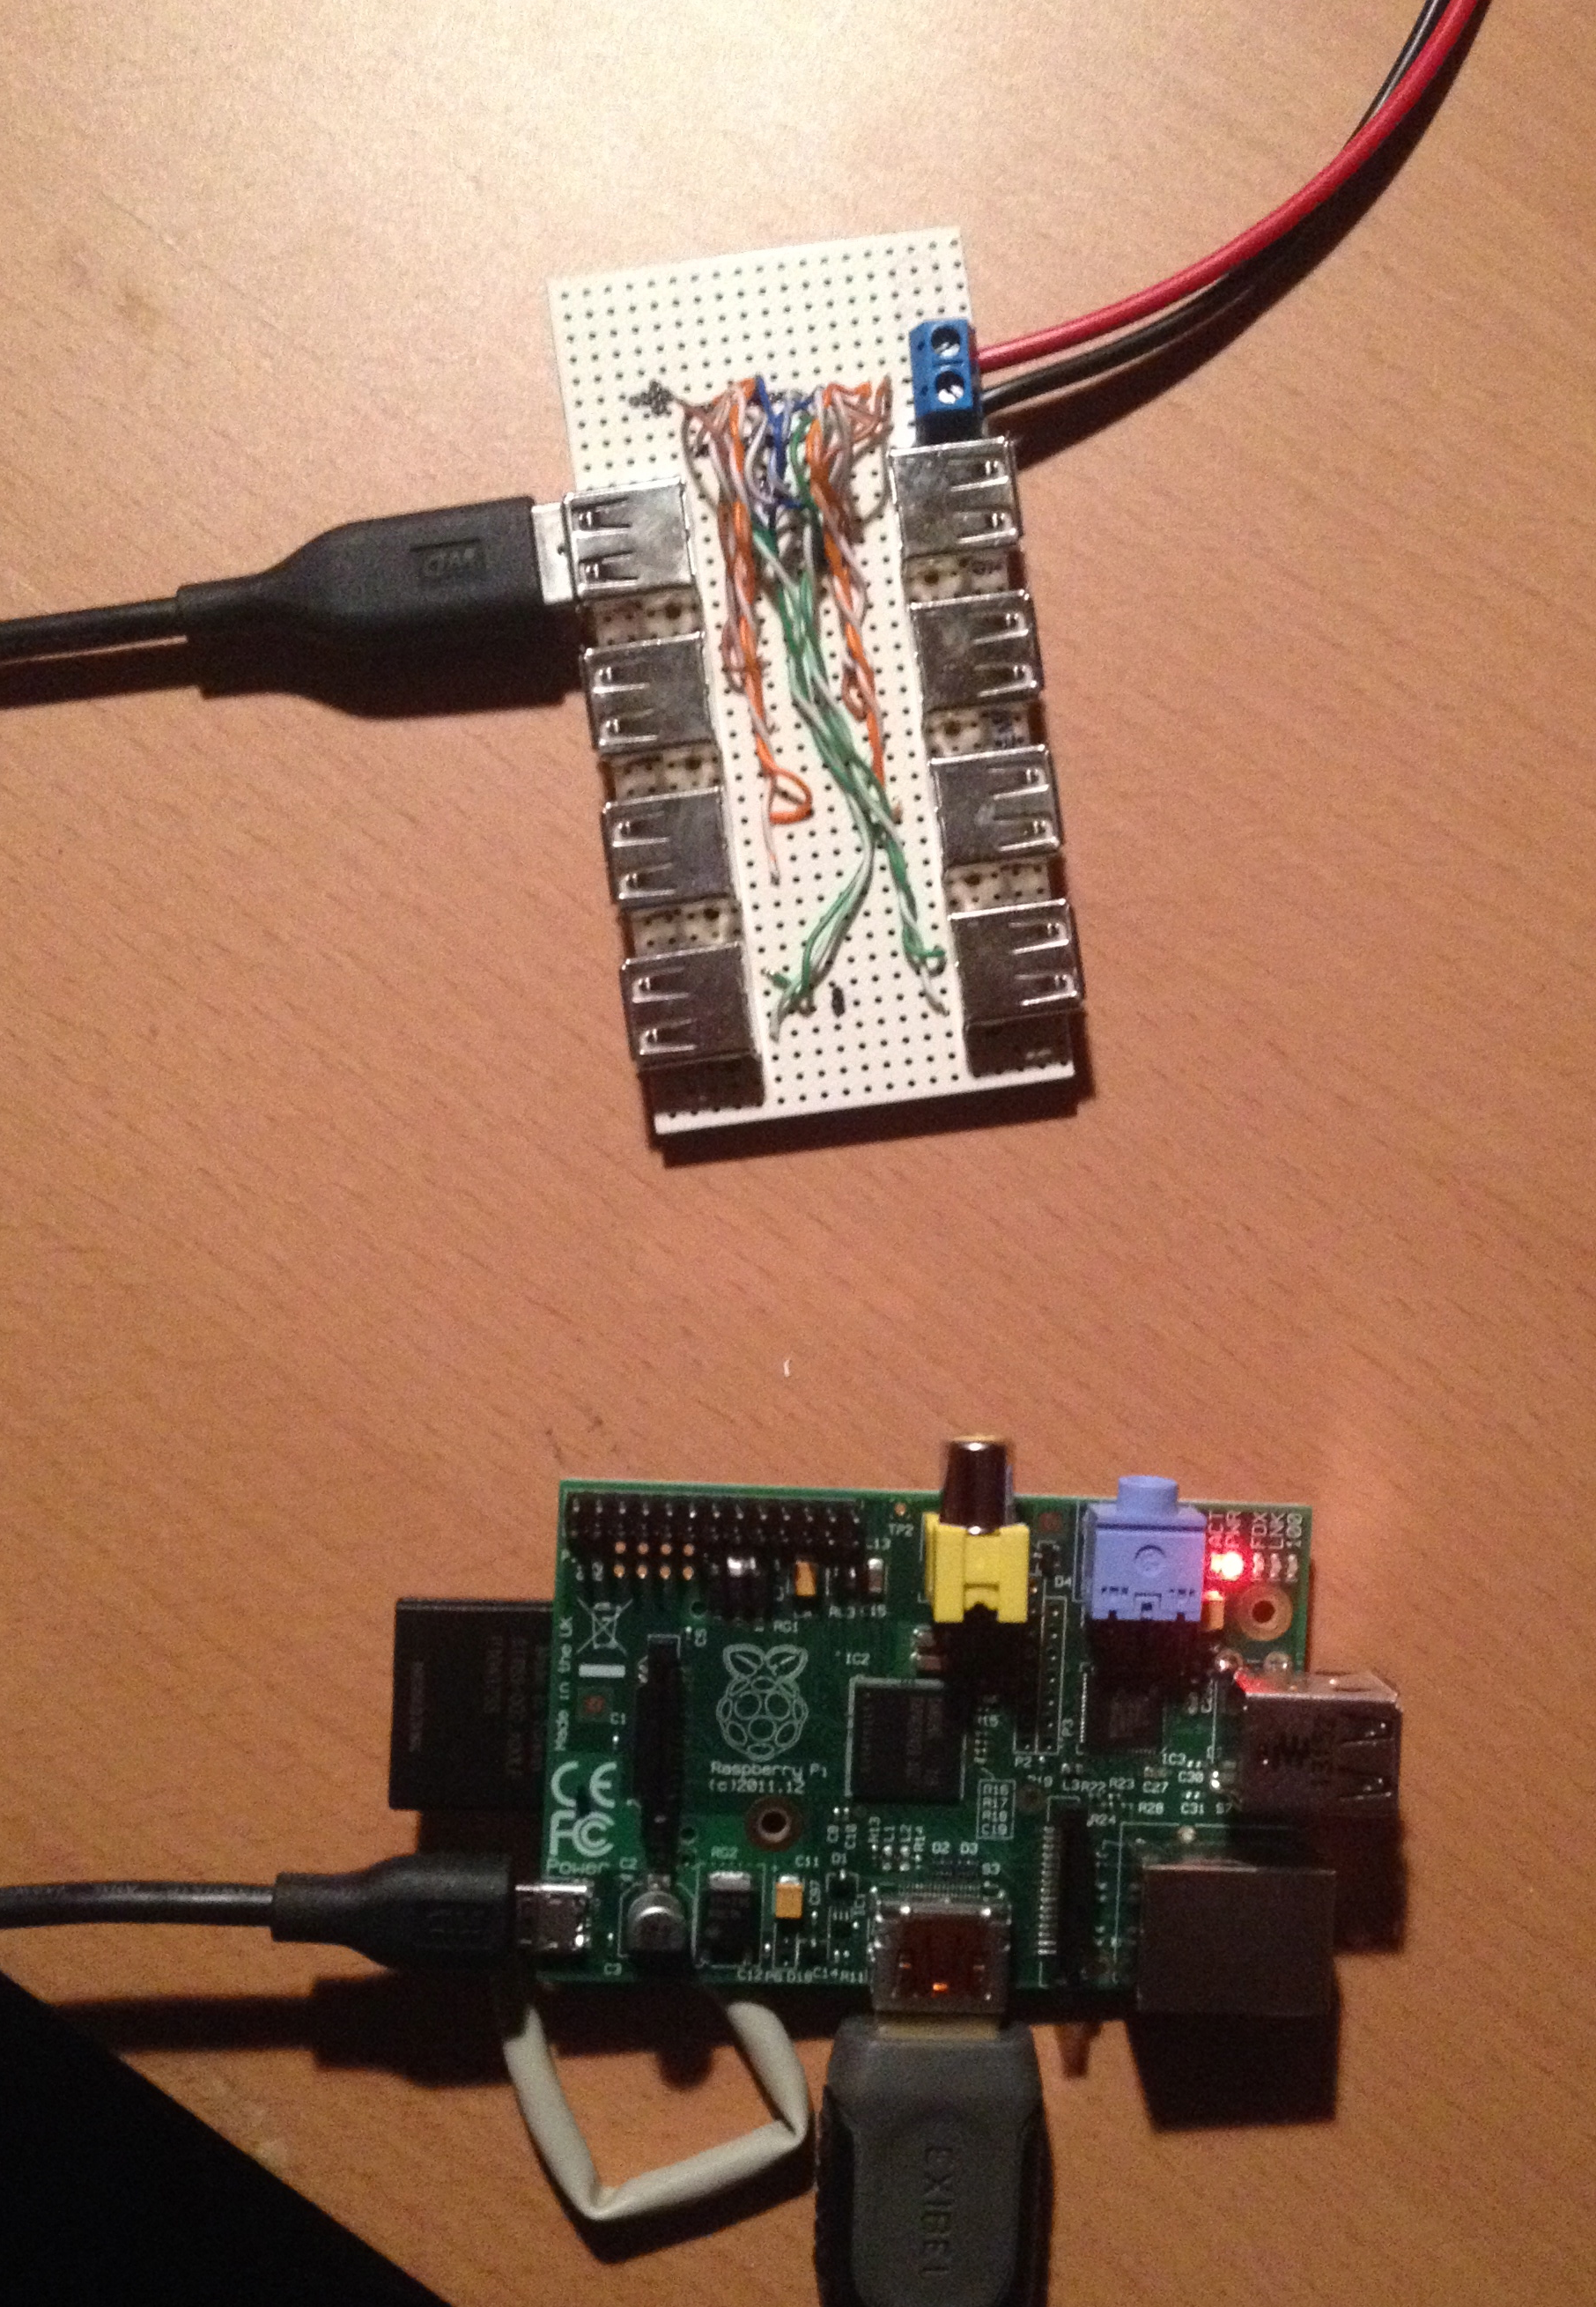
\includegraphics[width=0.5\textwidth]{thebuild/result.png}
    \caption{Power supply: end result}
    \label{fig:build_power_supply}
\end{figure}

\subsection{The cluster}
Early in our project we only used a few of the Pis for proof of concept style work. When working with three or more nodes we quickly realized things were getting out of hand. We needed some form of structure to hold them to prevent clutter and avoid accidentally damaging them. After brainstorming ideas and some research we ended up with three options. 

We could buy stackable cases for the Raspberry PIs. This would be a costly but very practical solution. There are numerous web sites selling these kinds of cases. The cost for these cases are typically almost half the price of the PIs. So it would increase the cost of the cluster considerably.

Another interesting solution that we arguably discovered too late was building cases out of Lego. This was inspired by the Southampton University making a 64 node cluster using Lego as a frame for their structure.\cite{legos} 

The third option and the one we settled with was building our own structure. There are two ways to stack Raspberry PIs. Either you have some form of external skeleton and stack them on top of each other or you use spacing screws in the two mounting holes on the circuit board and screw them on top of each other. 

We bought a toolkit inlay in plastic from Clas Ohlson and a set of spacing screws in plastic from Ebay. Then drilled holes mounting holes in the bottom of the inlay and mounted 4 and 4 Raspberry PIs using the spacing screws. We secured the bottom spacer using nuts and discs. This left the other side of the inlay for the power supply and switch. In the end we were left with a very mobile cluster. 

\begin{figure}[h]
    \centering
    \includegraphics[width=0.5\textwidth]{thebuild/cluster_inside.jpg}
    \caption{Inside the clusterbox}
    \label{fig:build_cluster_inside}
\end{figure}

\begin{figure}[h]
	\centering
    \includegraphics[width=0.5\textwidth]{thebuild/cluster_under.jpg}
    \caption{Under the clusterbox}
    \label{fig:build_cluster_under}
\end{figure}

\begin{figure}[h]
    \centering
    \includegraphics[width=0.5\textwidth]{thebuild/raspberrypi_mounting_holes.png}
    \caption{Scheme showing mounting wholes}
    \label{fig:build_cluster_inside}
\end{figure}

\begin{figure}[ht]
\centering
\begin{minipage}[b]{0.45\linewidth}
    \includegraphics[width=1\textwidth]{thebuild/cluster_back.jpg}
    \caption{Back of the cluster}
    \label{fig:minipage1}
\end{minipage}
\quad
\begin{minipage}[b]{0.45\linewidth}
    \includegraphics[width=1\textwidth]{thebuild/cluster_front.jpg}
    \caption{Front of the cluster}
    \label{fig:minipage2}
\end{minipage}
\end{figure}

\subsection{Network equipment}
We were able to acquire network cables from the faculty, however they were all of various lengths. In order to have a neat system they would need to be shortened. So we cut the cables into appropriate lengths of around 30 cm, and used a crimping tool to fasten new connectors at the ends. This is a very cost effective way of making shorter cables. 

\begin{figure}[h]
    \centering
    \includegraphics[width=0.5\textwidth]{thebuild/tp_cable.jpg}
    \caption{The process of making a short TP-cable}
    \label{fig:build_tp_cable}
\end{figure}


